\documentclass[04.3_buildingProcess.tex]{subfiles}
\begin{document}
    \subsubsection{Conductive Ink Process}
    \begin{flushleft}
        \noindent
        In addition to this, conductive ink \cite{conductiveInk} on the wood has been tested and if there is 
        still enough conductivity. The result is that the microcontroller can notice a 
        change; however, the resistance was between 1.7k\si{\ohm} and 12.2M\si{\ohm}, 
        so an analog pin has to be used to detect the current. In addition, a threshold has to be found, so 
        the system can detect if a leaf coupe is connected (see Figure \ref{fig:leaveConductiveInk}).

        \begin{figure}[h!]
            \centering
            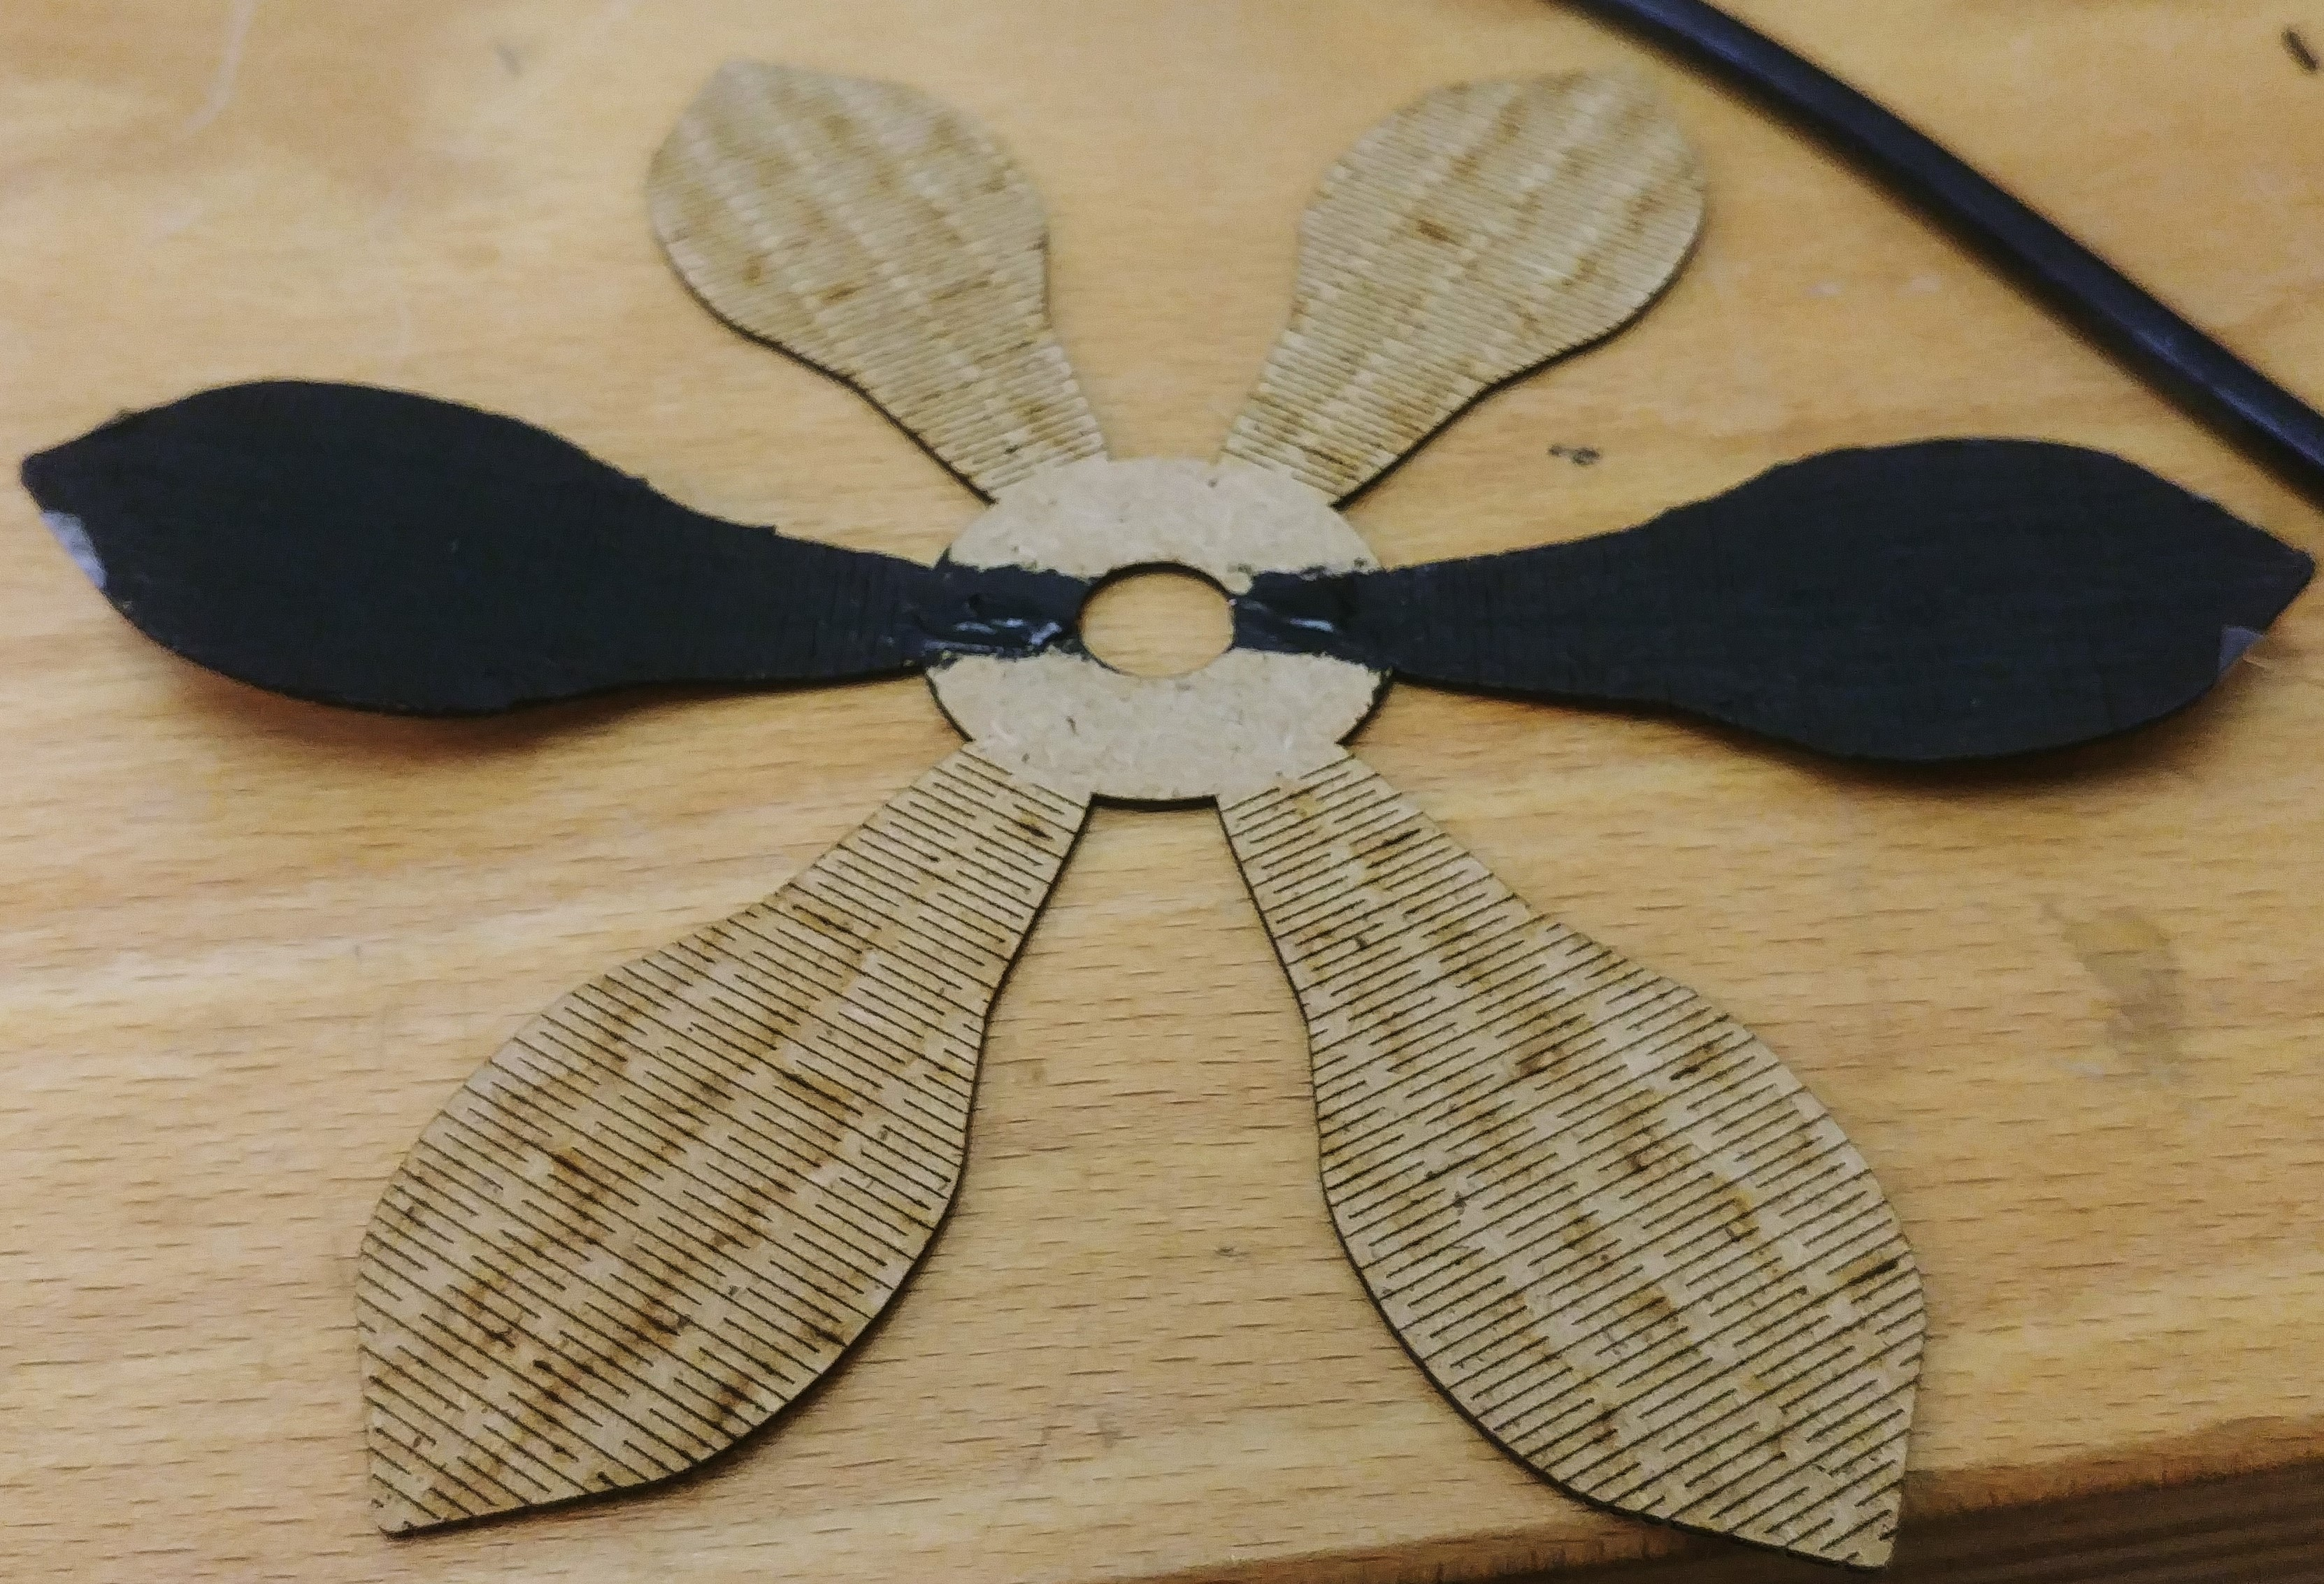
\includegraphics[scale=0.05]{images/materialProcess/leaveTesting_.jpg}
            \caption{Shows the testing of the conductive ink with wood.}
            \label{fig:leaveConductiveInk}
        \end{figure}

        \noindent
        After the conductive test (see Figure \ref{fig:leaveConductiveInk}), conductive ink has been 
        printed on wood before laser cutting. Before, the company of the ink has been messaged and asked 
        if there is something inside the paint that burns or is toxic. The cutting patter had to be changed 
        because the ink burns stronger than the wood itself, so it burned parts of the leaves. 
        That's why the distance of the cuts had to be increased(see Figure \ref{fig:07_LaserCut}). 

        \begin{figure}[h!]
            \centering
            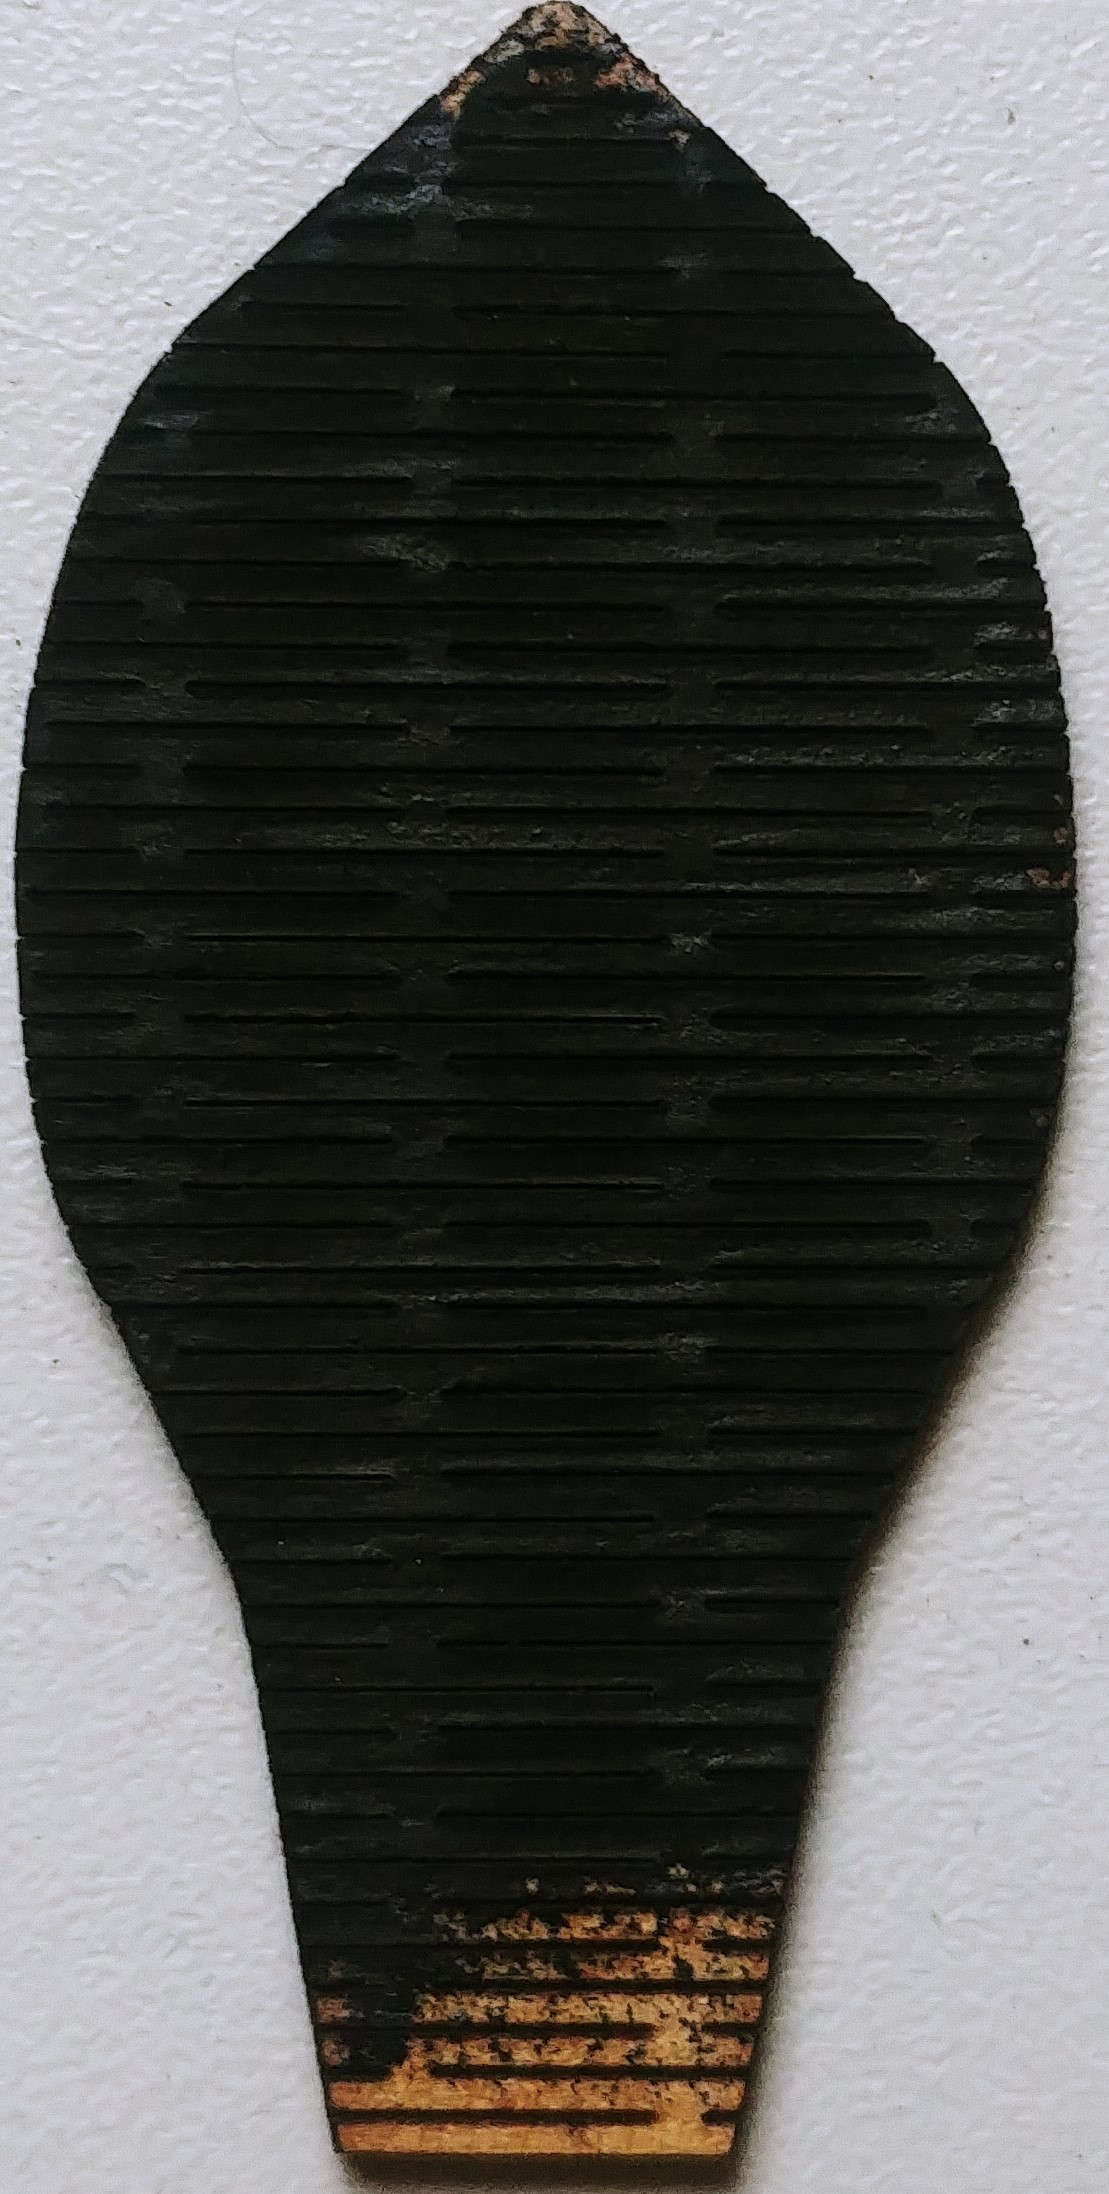
\includegraphics[scale=0.05]{images/materialProcess/07_LaserCut.jpg}
            \caption{Shows the result of the laser cut with capacitive ink on wood.}
            \label{fig:07_LaserCut}
        \end{figure}

        \noindent
        However, even after this success of cutting a test shape with conductive ink, the flexibility
        couldn't be increased without increasing the size of the shape. However, somehow the flexibility 
        had to increase because of the LEDs in the middle of the base and the light ball. 
        The diameter of the light ball is 3 centimeters. The overcome of this diameter was a problem
        and could not be solved in time, so cork was the choice instead. This material is very flexible, even 
        without cuts (see Figure \ref{fig:corkTest}).\\

        \begin{figure}[H]
            \centering
                \includegraphics[scale=0.05]{images/materialProcess/corkBlossomShape.jpg}
                \caption{Shows the corc blossom shape cut that will be used for the final prototype.}
                \label{fig:corkTest}
        \end{figure}
    \end{flushleft}
\end{document}